\documentclass[times, utf8, zavrsni, english]{fer}
\usepackage{booktabs}
\usepackage{graphicx}
\graphicspath{ {./images/} }

\begin{document}

% TODO: Navedite broj rada.
\thesisnumber{000}

% TODO: Navedite naslov rada.
\title{Application of NLP to threat classification from cybersecurity records}

% TODO: Navedite svoje ime i prezime.
\author{Mirta Medak}

\maketitle

% Ispis stranice s napomenom o umetanju izvornika rada. Uklonite naredbu \izvornik ako želite izbaciti tu stranicu.
\izvornik

% Dodavanje zahvale ili prazne stranice. Ako ne želite dodati zahvalu, naredbu ostavite radi prazne stranice.
\zahvala{}

\tableofcontents

\chapter{Introduction}
Every entity that is dependent on a computer system, from corporations to individuals, could be a subject to cyber attacks. \\
In 2018 there were 80,000 cyber attacks per day or over 30 million attacks per year. [1] During the CoVid-19 pandemic, the cybercrime went up 600, as PurpleSec suggests. [2] \\
As technology evolves, more various threats to its security emerge.
Tracking, describing, and evaluating these threats is of use when developing defense systems and making business decisions. \\

\section{Common Vulnerabilities and Exposures System}
A \textbf{vulnerability} is a weakness in a computer system, that can be exploited by an attacker to execute malicious commands, access data in an unauthorized way, or perform other types of cyber attacks. [4,5] \\
A \textbf{threat} is any circumstance or event which has the potential to compromise system security. [6] \\
In order to tackle the cybersecurity problems in a more organized manner, a system of \emph{CVE (Common Vulnerability and Exposure)} has been developed. \\
The \emph{MITRE Corporation} maintains a public database of an increasing number of CVE records. \\
A CVE record includes an ID, a brief description of the vulnerability, and references.

\section{Common Vulnerability Scoring System}
In order to manipulate and prioritize vulnerabilities in a system, the metric of the Common Vulnerability Scoring System (CVSS) score is used. This metric estimates how "dangerous" an exploitation of a vulnerability is. CVSS is an emerging standard of vulnerability comparison. [8] \\
CVSS is divided in three groups: \emph{Base, Temporal and Environmental score}. 
\textbf{Base Score} group shows the traits of the vulnerability that do not change over time and are not dependent on the environment. [9] Predicting the base score will be the subject of this research. \\

\begin{figure}[h]
	\caption{There are eight CVSS Base submetrics:}
	\centering
	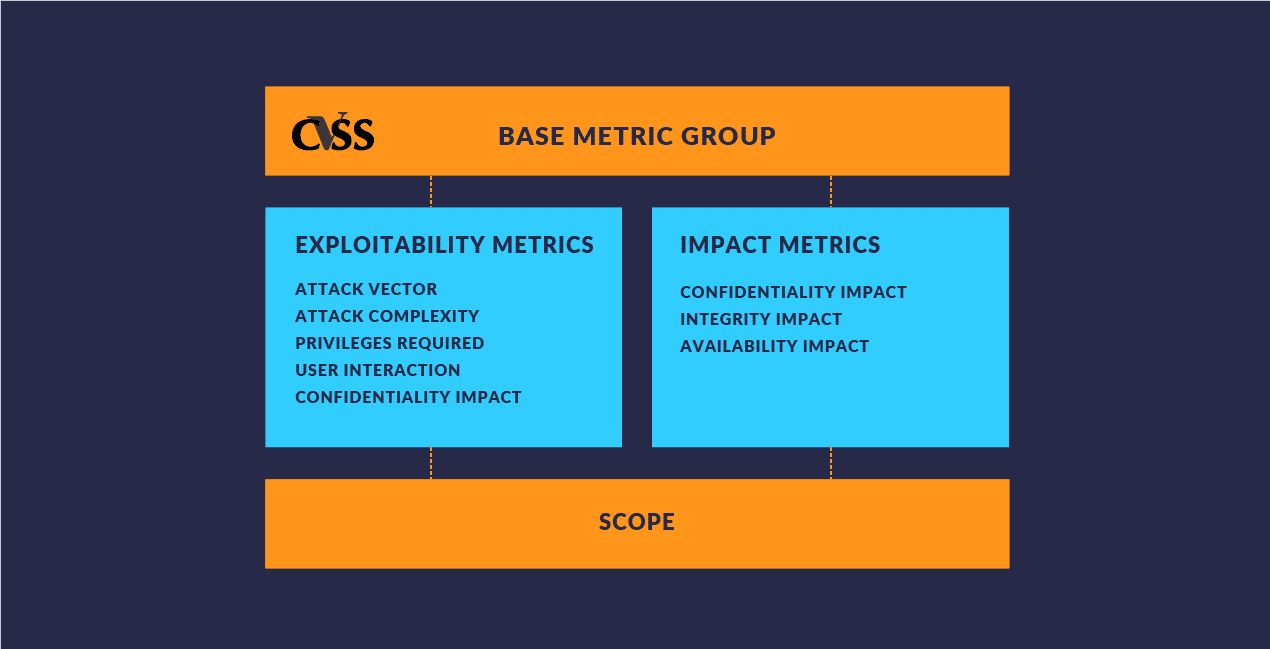
\includegraphics[scale=0.25]{CVSS-Base-Metric-Group}
\end{figure}
Each submetric is assigned by experts. E. g., attack complexity can be assigned as High or Low. From these submetrics a hard-coded formula is used to compute the final Base score. \\
Atefeh Khazaei et al. show an important concern in their work [8]: the CVSS calculation \textbf{can be subjective}.
Moreover, the annotation requires experts and time, which is prolonging the process and is costly. \\
\\

In this research, NLP methods are used to predict the CVSS Base score by analyzing the description from the CVE record.

\chapter{Related work}


\chapter{Data}

\chapter{Models}

\chapter{Experiments and results}

\chapter{Conclusion}
Conclusion.

\bibliography{literatura}
\bibliographystyle{plainnat}

\listoffigures
\begin{abstract}
Abstract.

\keywords{Keywords.}
\end{abstract}

% TODO: Navedite naslov na hrvatskom jeziku.
\hrtitle{Naslov}
\begin{sazetak}
Sažetak na hrvatskom jeziku.

\kljucnerijeci{Ključne riječi, odvojene zarezima.}
\end{sazetak}

\end{document}
